Empleando el montaje descrito, se obtuvo la curva presentada en la \cref{fig:graph},
donde se muestra la corriente del circuito en función del potencial de aceleración.
Para la medición, se empleó un potencial de corrección \( U_1 = \qty{4.16}{\volt} \)
y un potencial de frenado \( U_3 = \qty{0.24}{\volt} \).

\begin{figure}[htbp!]
  \centering
  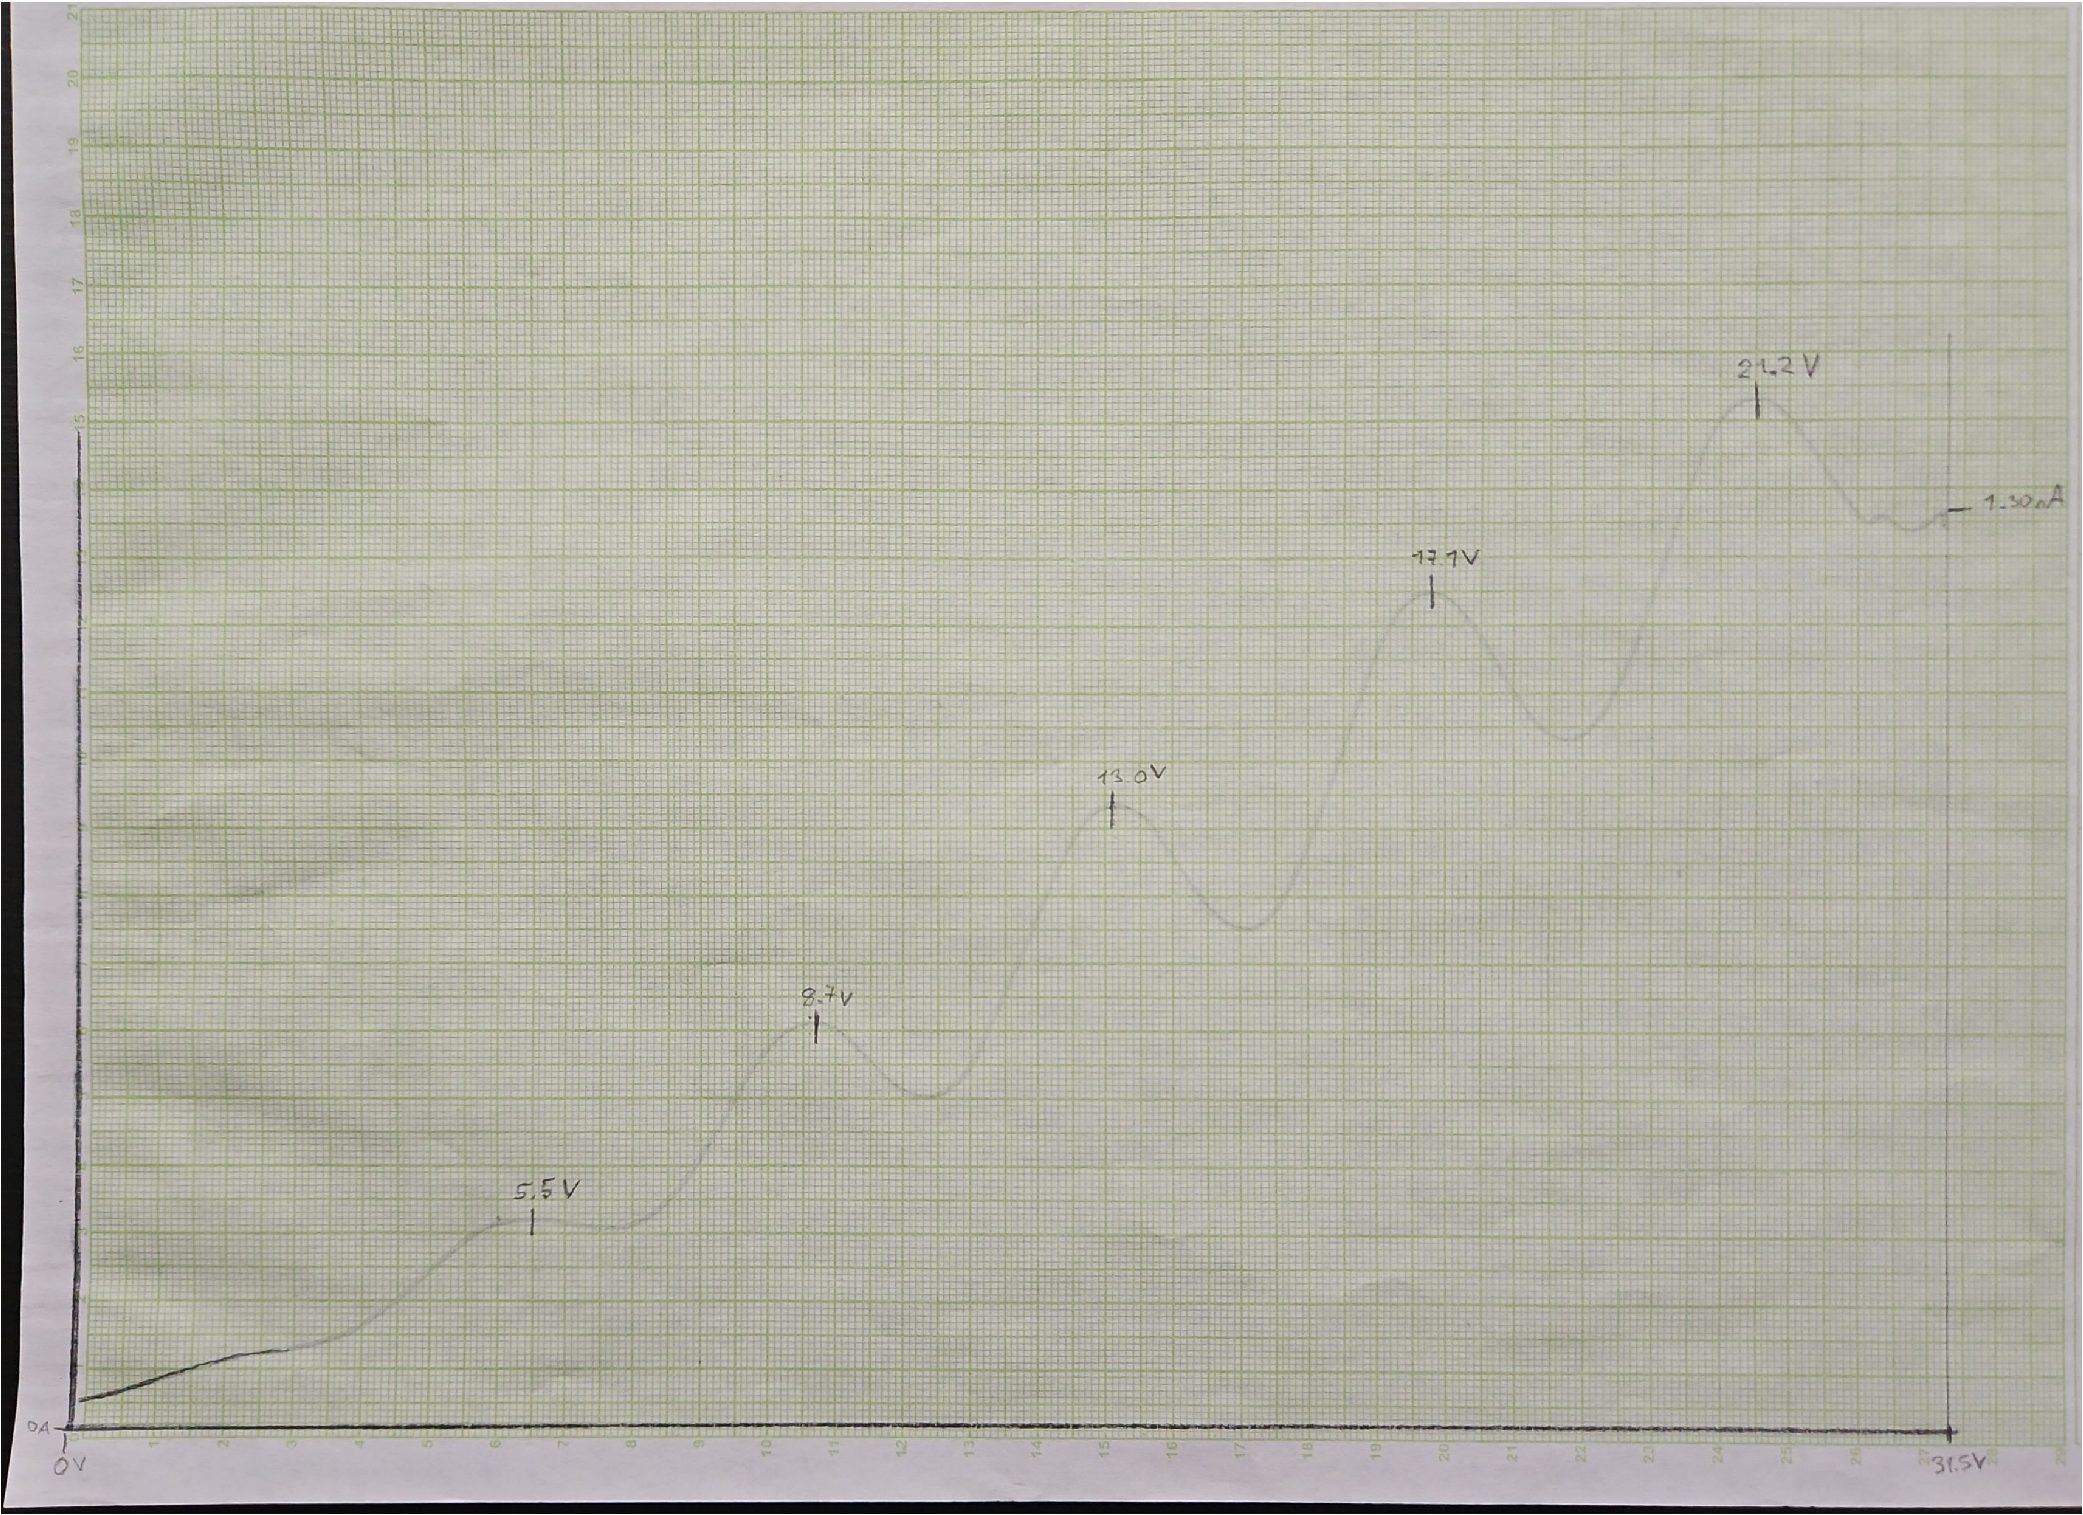
\includegraphics[width=0.9\linewidth]{./Figures/Graph-Scan.pdf}
  \caption{Gráfica obtenida con el osciloscopio.}
  \label{fig:graph}
\end{figure}

Se observa que la corriente no sigue un comportamiento lineal.
Inicialmente, aumenta con el potencial hasta alcanzar un valor máximo,
tras lo cual decrece y luego vuelve a incrementarse.
Los picos de corriente y sus respectivos valores de potencial
se presentan en la \cref{tab:peaks}, donde se obtiene una separación
promedio entre picos de \( \Delta U = \qty{5.2}{\volt} \).
Se registró una corriente final de \qty{1.30}{\nano\ampere} y un
máximo de \qty{1.45}{\nano\ampere}.

\begin{table}[htbp!]
  \centering
  \pgfplotstabletypeset[
  col sep=tab,
  text indicator=", string type,
  header=false,
  zerofill,
  columns={0,1},
  columns/0/.style={
    column name={\text{\( U \) \([\si{\volt}]\)}},
    column type={S[table-format=2.1]}
  },
  columns/1/.style={
    column name={\text{\( I \) \([\si{\nano\ampere}]\)}},
    column type={S[table-format=1.2]},
  },
  every even row/.style={
    before row={\rowcolor[gray]{0.95}},
  },
  every head row/.style={
    before row=\toprule, after row=\midrule},
  every last row/.style={
    after row=\bottomrule,
  },
  ]{./Data/peaks-current.tsv}
  \vspace{1.5pt}
  \caption{Valores experimentales de los picos de corriente.}
  \label{tab:peaks}
\end{table}


El valor esperado de separación entre picos es \qty{4.9}{\volt},
lo que representa un error relativo del \qty{7.54}{\percent}
respecto a la separación promedio obtenida en el experimento.
